\documentclass[11pt,a4paper]{article}

\usepackage[margin=1in]{geometry}
\usepackage{graphicx}
\usepackage{float}
\usepackage{amsmath}
\usepackage[utf8]{inputenc}
\usepackage[T1]{fontenc}
\usepackage{lmodern}
\usepackage{microtype}
\usepackage{csquotes}
\usepackage[spanish]{babel}
\usepackage{cite}
\usepackage{listings}
\usepackage{xcolor}
\usepackage{caption,subcaption}
\usepackage{booktabs}
\usepackage[hidelinks]{hyperref}

\lstset{
    basicstyle=\ttfamily\small,
    keywordstyle=\color{blue},
    commentstyle=\color{gray},
    breaklines=true
}
 
\makeatletter
% allow a subtitle
\providecommand\@subtitle{}
\newcommand{\subtitle}[1]{\gdef\@subtitle{#1}}

% provide a way to set two author emails
\providecommand\@emailone{email1@example.com}
\providecommand\@emailtwo{email2@example.com}
\newcommand{\authoremails}[2]{\gdef\@emailone{#1}\gdef\@emailtwo{#2}}

% default subtitle and emails (editable)
\subtitle{Máster en Inteligencia Artificial - Universidad de Murcia}
\authoremails{jdiego.gallego@um.es}{oscar.veral@um.es}

% Redefine \maketitle to produce a dedicated titlepage
\renewcommand{\maketitle}{%
    \begin{titlepage}
        \centering
        \thispagestyle{empty}
        \vspace*{2.5cm}
        {\Huge\bfseries\@title\par}
        \vspace{1cm}
        {\Large\itshape\@subtitle\par}
        \vspace{3cm}
        {\large
            \begin{tabular}{c}
                \@author
            \end{tabular}\par
        }
        \vspace{0.6cm}
        {\small
            \begin{tabular}{c}
                \texttt{\@emailone} \\[0.8ex]
                \texttt{\@emailtwo}
            \end{tabular}\par
        }
        \vfill
        {\large \@date\par}
    \end{titlepage}%
}
\makeatother

\begin{document}

\title{Informe BT3 y BT4\\[1ex]\large Visión Artificial}
\author{Juan Diego Gallego Nicolás \and Óscar Vera López}
\date{\today}

\maketitle

\renewcommand{\contentsname}{Índice}
\setcounter{tocdepth}{3}
\tableofcontents
\clearpage


\section*{Introducción}
En este informe se detallan las implementaciones y resultados obtenidos en las tareas de procesamiento de imágenes realizadas para los bloques de trabajo BT3 y BT4.
Todas las referencias a código fuente, notebooks y datos se encuentran en el repositorio de GitHub asociado al proyecto: \href{https://github.com/oscarveral/vision}{vision}

\section*{Items cubiertos}
\begin{itemize}
  \item \textbf{BT3a}: Comparación de detectores y extractores de descriptores locales (SIFT u otros).
  \item \textbf{BT3b}: Matching entre imágenes.
  \item \textbf{BT3c}: Estimación robusta de transformaciones.
  \item \textbf{BT3kp}: Implementación de un clasificador HOG+SVM para detección de señales de tráfico.
\end{itemize}

\section{BT3: Hand-engineered features y reconocimiento robusto de objetos}

En esta sección se describe las tecnicas aplicadas para la detección y reconocimiento de señales de tráfico en imágenes utilizando descriptores locales y 
métodos de matching robustos. Partimos del dataset ya mencionado anteriormente, en el que disponemos de 
imágenes de escenas de conducción en diferentes entornos, además de toda la infraestructura desarrollada
para el procesamiento de imágenes.

\subsection{Extracción de descriptores locales}

\textit{Items de evaluación: \underline{\textbf{BT3a}},
\underline{\textbf{BT3b}}.}

Manteniendo la misma metodología de desarrollo seguida hasta ahora,
hemos desarrollado una clase \texttt{LocalDescriptorExtractor} que 
nos permite extraer los descriptores locales de una imagen dada usando 
diferentes técnicas. En nuestro caso, implementamos tanto AKAZE como SIFT y 
ORB, utilizando las implementaciones disponibles en OpenCV.

De momento trabajaremos con el mismo set de imágenes de prueba que se ha 
utilizado en los bloques anteriores, que contienen señales de tráfico en 
distintas condiciones de iluminación y entornos. EL objetivo de esta sección 
es comparar el rendimiento de los diferentes descriptores locales en el 
matching de entre imágenes del dataset y dichas imágenes transformadas.

Utilizando nuestro extractor, hemos creado una visualización \ref{fig:keypoints_comparison} de los puntos clave
detectados con cada método en una imagen de prueba representativa:

\begin{figure}[H]
    \centering
    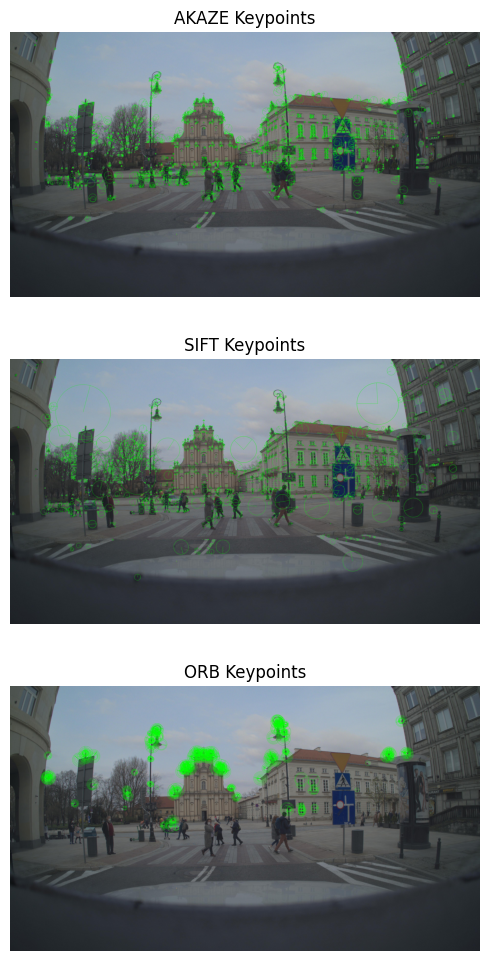
\includegraphics[width=0.6\textwidth]{images/keypoints_comparisons.png}
    \caption{Comparación de puntos clave detectados por diferentes descriptores locales.}
    \label{fig:keypoints_comparison}
\end{figure}

Observese cómo varían los puntos clave detectados por cada método 
en la misma imagen. Akaze tiende a detectar más puntos clave de
forma más exhaustiva, mientras que SIFT es algo más general y ORB es 
mucho menos preciso, 
enfocándose en puntos de interés muy generales y quizás menos 
precisos. Es interesante entonces observar como pueden influenciar
transformaciones arbitrarias en la detección de puntos clave según
el método empleado. Para ello, nos valemos de nuestro procesador 
de imagenes para aplicar diferences transformaciones y observar 
los resultados.

\begin{figure}[H]
    \centering
    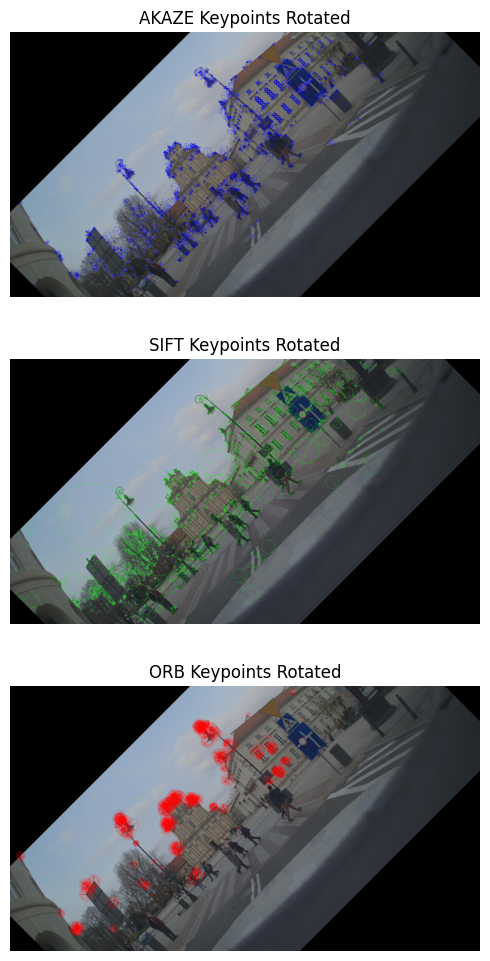
\includegraphics[width=0.6\textwidth]{images/keypoints_rotated.png}
    \caption{Comparación de puntos clave detectados con rotación.}
    \label{fig:keypoints_rotated}
\end{figure}

Visualmente, se aprecia como se mantienen correctamente los puntos 
clave detectados tras la rotación. Veamos numericamente los resultados
para obtener conclusiones más precisas y una representación 
visual del matching entre puntos realizado. 
 
Para calcular las estadísticas de matching, se ha utilizado un 
matcher de fuerza bruta, aplicando la ratio test de Lowe\cite{lowe} para 
filtrar los matches incorrectos. Esta técnica de filtrado se basa 
en buscar el descriptor más cercano en la segunda imagen para cada 
descriptor de la primera. Para evitar falsos positivos, se compara la 
distancia del descriptor más cercano con la del segundo descriptor 
más cercano. Si la relación entre estas dos distancias es menor que 
un umbral predefinido (comúnmente 0.75), se considera que el match es 
válido. Esta técnica ayuda a mejorar la precisión del matching al 
reducir la probabilidad de emparejamientos incorrectos.

La metodología seguida ha sido la siguiente:
\begin{itemize}
    \item Selección de una imagen de prueba representativa del dataset.
    \item Aplicación de una transformación básica.
    \item Extracción de descriptores locales en ambas imágenes.
    \item Matching de descriptores entre ambas imágenes.
    \item Cálculo del número de matches que satisfacen Lowe y tasa de repetibilidad (matches buenos / puntos clave originales).
\end{itemize}

Los resultados obtenidos a continuación se han mantenido con poca variación
al repetir el experimento con distintas imágenes de prueba del dataset. Exponemos
aquí sólo un caso representativo.

Para una rotación como la mostrada en la figura \ref{fig:keypoints_rotated},
los resultados obtenidos son los siguientes:
\begin{itemize}
    \item \textbf{AKAZE}: 
    \begin{itemize}
        \item Puntos clave originales: 4278.
        \item Puntos clave rotados: 3730.
        \item Matches: 3186.
        \item Matches tras ratio test: 2856.
        \item Tasa de repetibilidad: 66.7\%.
        \item Tiempo de extracción: 0.72s.
    \end{itemize}
    \item \textbf{SIFT}:
    \begin{itemize}
        \item Puntos clave originales: 6641.
        \item Puntos clave rotados: 5552.
        \item Matches: 4632.
        \item Matches tras ratio test: 4107.
        \item Tasa de repetibilidad: 61.8\%.
        \item Tiempo de extracción: 1.20s.
    \end{itemize}
    \item \textbf{ORB}:
    \begin{itemize}
        \item Puntos clave originales: 1000.
        \item Puntos clave rotados: 1000.
        \item Matches: 768.
        \item Matches tras ratio test: 630.
        \item Tasa de repetibilidad: 63.0\%.
        \item Tiempo de extracción: 0.05s.
    \end{itemize}
\end{itemize}

Nótose que en nuestra implementación hemos tratado los puntos clave que 
se han matcheado de form que un punto clave original sólo puede matchearse
con un punto clave transformado. Esto puede reducir el número de matches
obtenidos, pero permite un calculo fiable de la tasa de repetibilidad.
No tiene sentido en este tipo de análisis que un punto clave original
matchee con varios puntos clave transformados, sobre todo si no estamos
aplicando en nuestro dominio transformaciones que puedan generar
duplicados (como reflejos o simetrías).

Los 3 métodos presentan tasas de repetibilidad similares y medianamente
altas, teniendo en cuenta que la rotación recorta la imagen. Akaze
presenta la tasa más alta, seguido de ORB y SIFT. En cuanto al tiempo
de extracción, ORB es con diferencia el más rápido, seguido de Akaze
y SIFT. Esto es esperable, ya que ORB está diseñado para ser un
método rápido y eficiente, aunque a costa de precisión. La figura
\ref{fig:matches_rotated} muestra una visualización de los matches
obtenidos entre la imagen original y la rotada para cada método.

\begin{figure}
    \centering
    \begin{subfigure}[b]{0.45\textwidth}
        \centering
        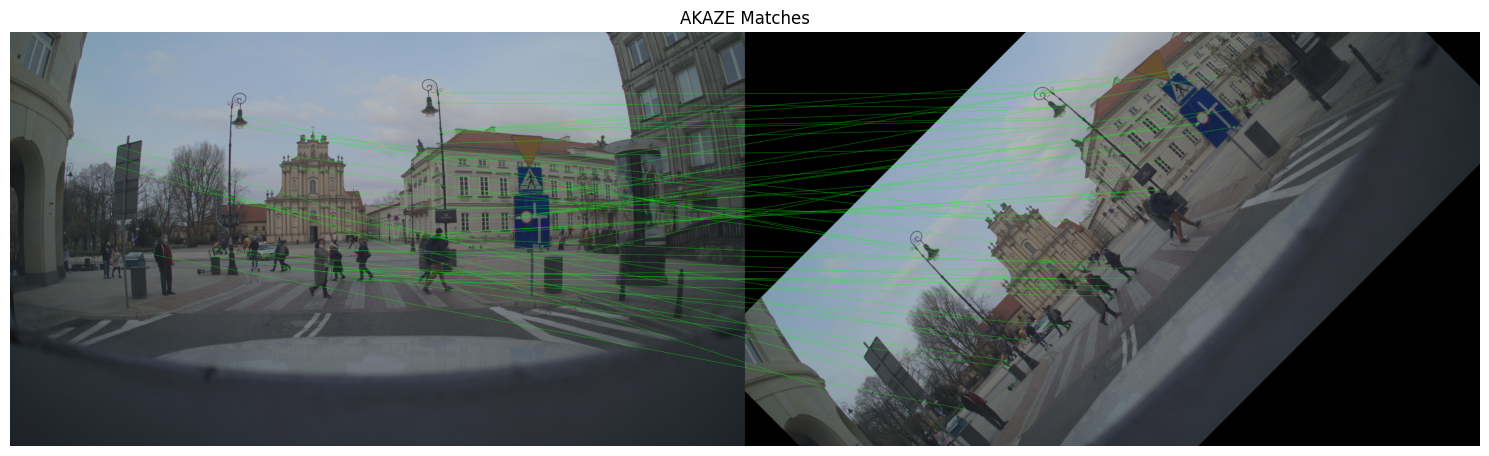
\includegraphics[width=\textwidth]{images/matching_akaze.png}
        \caption{AKAZE Matches}
    \end{subfigure}
    \hfill
    \begin{subfigure}[b]{0.45\textwidth}
        \centering
        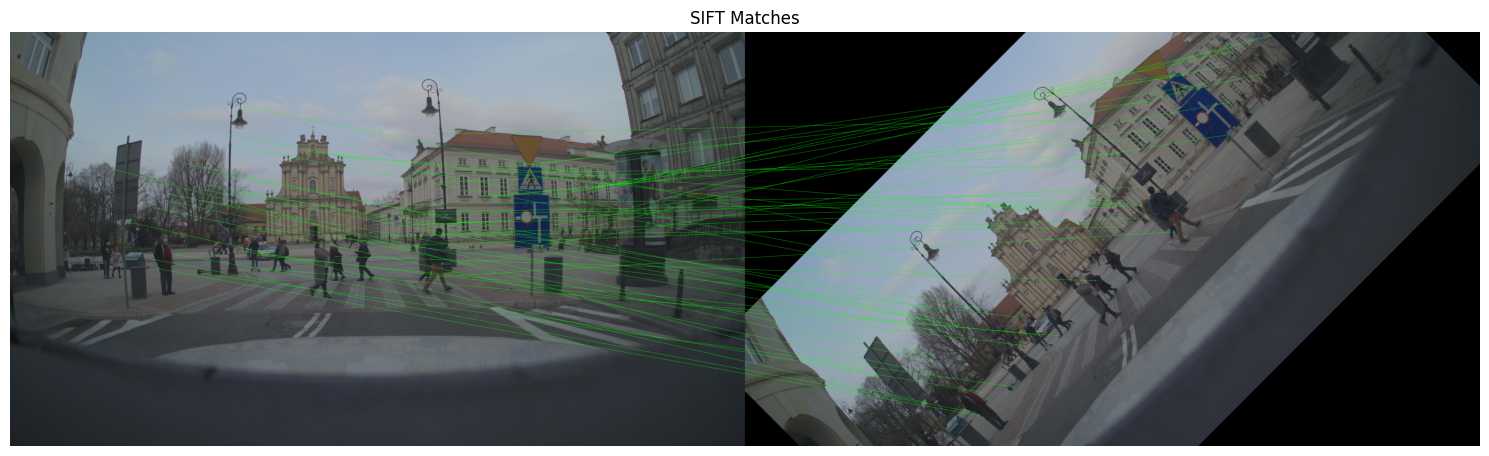
\includegraphics[width=\textwidth]{images/matching_sift.png}
        \caption{SIFT Matches}
    \end{subfigure}
    \hfill
    \begin{subfigure}[b]{0.45\textwidth}
        \centering
        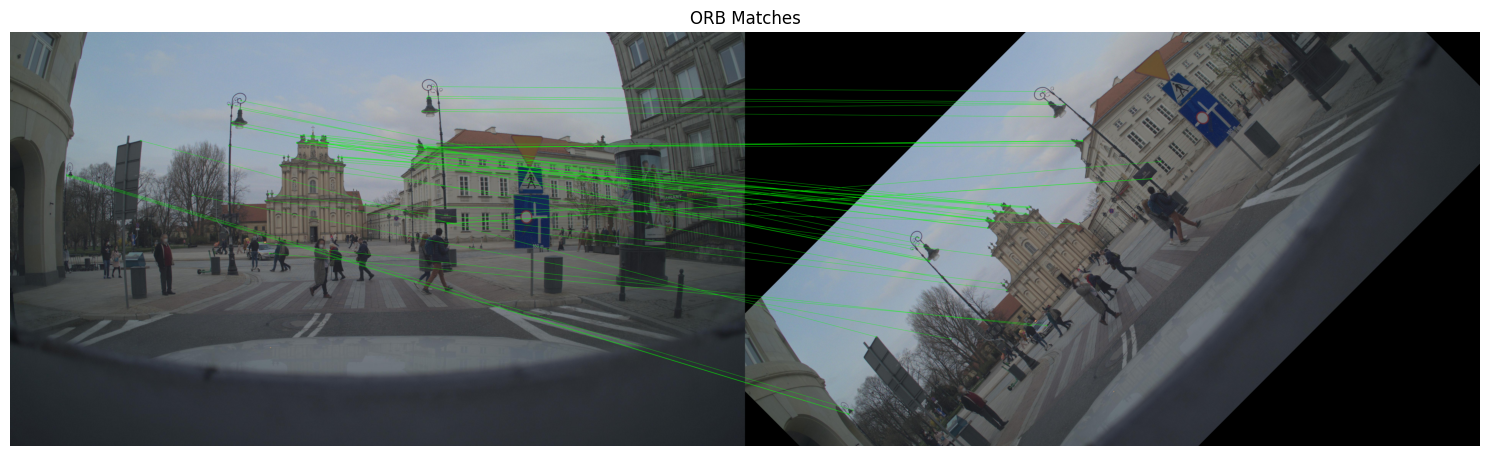
\includegraphics[width=\textwidth]{images/matching_orb.png}
        \caption{ORB Matches}
    \end{subfigure}
    \caption{Visualización de matches entre imagen original y rotada.}
    \label{fig:matches_rotated}
\end{figure}

Si aplicamos una transformación de ruido gaussiano, obtenemos la siguiente repetibilidad
para cada método:

\begin{itemize}
    \item \textbf{AKAZE}: 58.3\%.
    \item \textbf{SIFT}: 29.7\%.
    \item \textbf{ORB}: 44.4\%.
\end{itemize}

El ruido gausiano introducido ha sido muy fuerte ($\sigma=25$), lo que explica la caída
en la tasa de repetibilidad en SIFT. Aun así, generalmente se mantiene la robustez.
La figura \ref{fig:matches_noised} muestra una visualización de los puntos clave
originales y con ruido gaussiano para cada método.

\begin{figure}
    \centering
    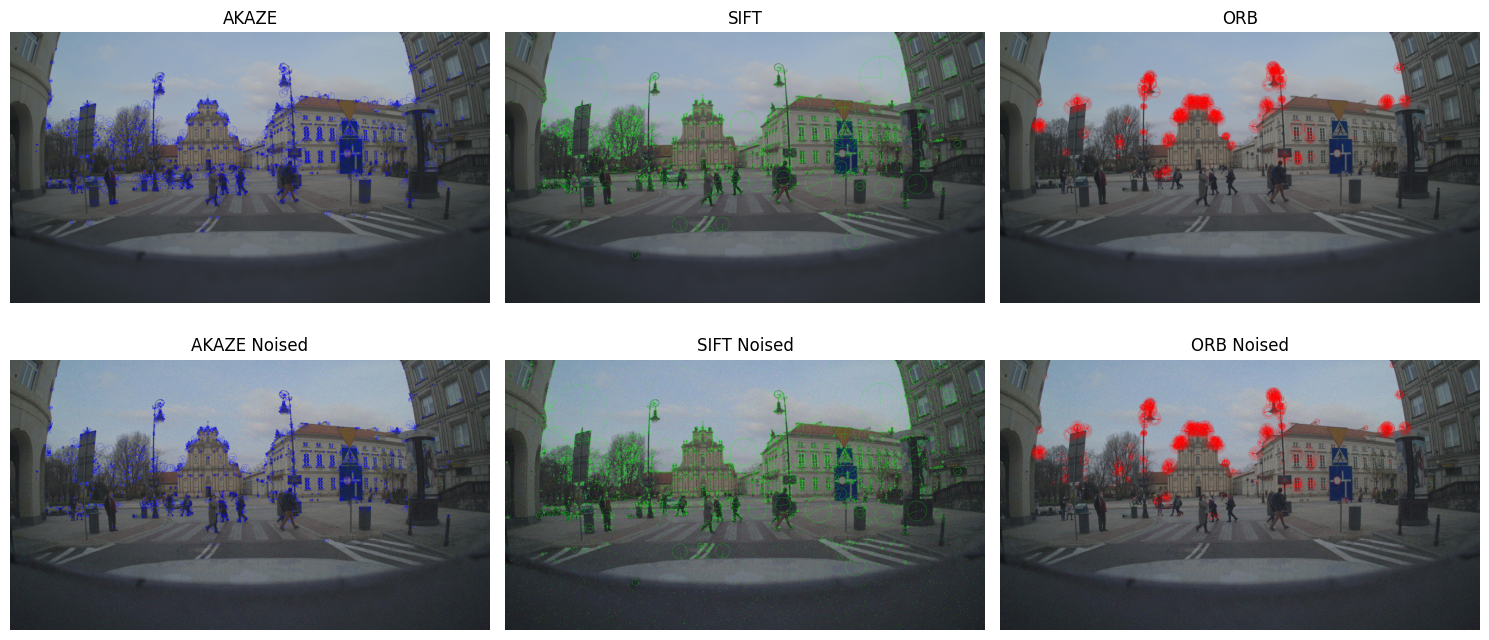
\includegraphics[width=0.6\textwidth]{images/matching_noised.png}
    \caption{Visualización de punts clave originales y con ruido gaussiano.}
    \label{fig:matches_noised}
\end{figure}

Probando con cambbios de escala obtenemos los siguientes resultados de repetibilidad:
\begin{itemize}
    \item \textbf{AKAZE}: 32.0\%.
    \item \textbf{SIFT}: 43.4\%.
    \item \textbf{ORB}: 23.66\%.
\end{itemize}

La tasa de repetibilidad cae en todos los casos, SIFT se alza ahora
como el método más robusto a cambios de escala. La figura \ref{fig:matches_scaled} muestra una 
visualización de los matches obtenidos entre la imagen original y la escalada para cada método.
Véase como, aunque la repetibilidad baja, visualmente los matches son casi perfectos entre
imagen original y escalada.
\begin{figure}
    \centering
    \begin{subfigure}[b]{0.45\textwidth}
        \centering
        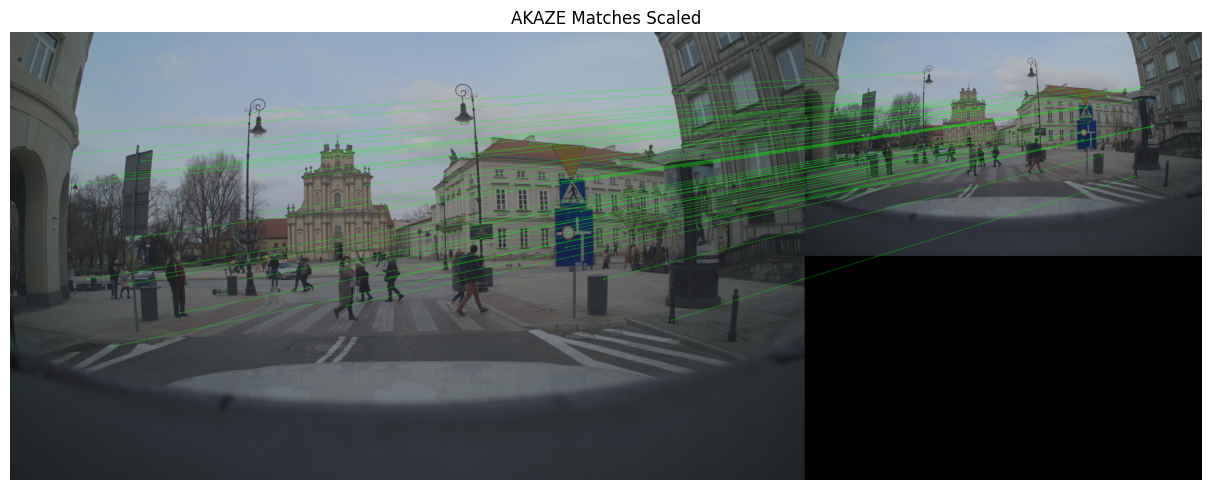
\includegraphics[width=\textwidth]{images/matching_akaze_scaled.png}
        \caption{AKAZE Scaled}
    \end{subfigure}
    \hfill
    \begin{subfigure}[b]{0.45\textwidth}
        \centering
        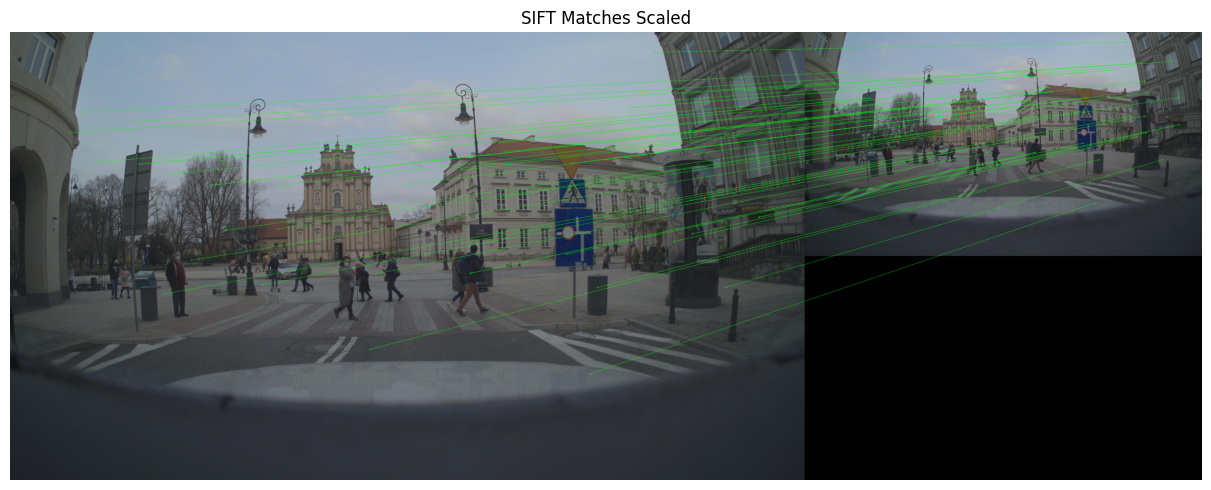
\includegraphics[width=\textwidth]{images/matching_sift_scaled.png}
        \caption{SIFT Scaled}
    \end{subfigure}
    \hfill
    \begin{subfigure}[b]{0.45\textwidth}
        \centering
        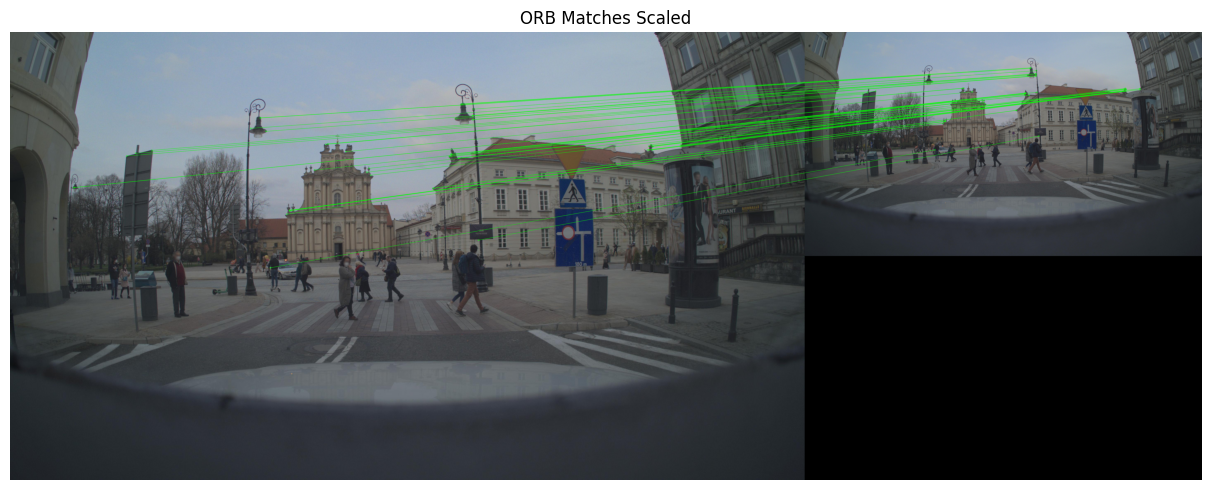
\includegraphics[width=\textwidth]{images/matching_orb_scaled.png}
        \caption{ORB Scaled}
    \end{subfigure}
    \caption{Visualización de matches entre imagen original y escalada.}
    \label{fig:matches_scaled}
\end{figure}

A partir de lo desarrollado, sería intersante obserbar los puntos clave
localizados en imágenes que han sido sometidas a transformaciones más complejas,
como puede serlo el mapeo al espacio HSV y la segmentación por color, 
que se desarrolló para la detección de bordes con RANSAC en BT1 y BT2.

Aplicar esta transformación hace que los algoritmos de extracción de
descriptores locales se focalizen en otras regiones de la imagen,
lo que nos interesa ya que ahora destacamos mejor las señales de tráfico.
La figura \ref{fig:matches_hsv} muestra los puntos clave detectados
en su transformación HSV y segmentación por color. Hablar de repetibilidad
en este caso no tiene sentido, ya que el objetivo de esta transformación
es precisamente cambiar el foco de atención de los detectores de puntos clave.

\begin{figure}
    \centering
    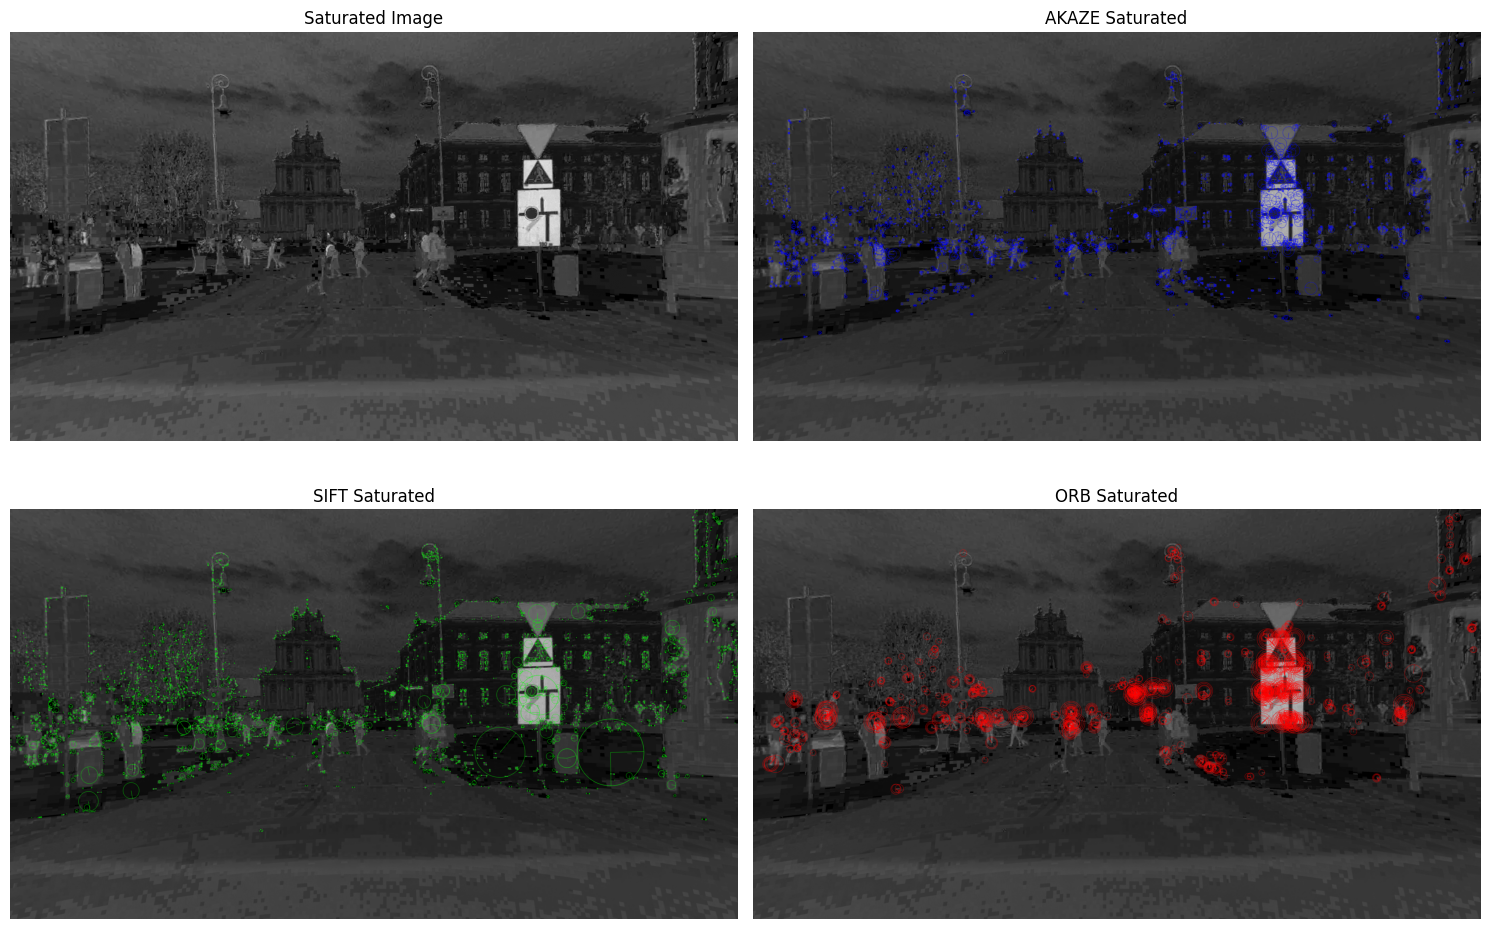
\includegraphics[width=0.6\textwidth]{images/keypoints_hsv.png}
    \caption{Visualización de punts clave en imagen HSV segmentada por color.}
    \label{fig:matches_hsv}
\end{figure}

Como apunte adicional, en nuestros experimentos, hemos observado también como las tecnicas
de contraste dinamico (CLAHE) permite mejorar un poco más el matching
entre imágenes, al resaltar mejor las regiones de interés. 

Como prueba final se ha aplicado una transformación compuesta más compleja,
que ha incluido la corrección de distorsión de la camara, contraste dinámico,
rotación de 30 grados, escalado al 75\% y ruido gaussiano ($\sigma=15$).

Los resultados visuales con SIFT son bastante satisfactorios, véase
la figura \ref{fig:matches_complex}.

\begin{figure}
    \centering
    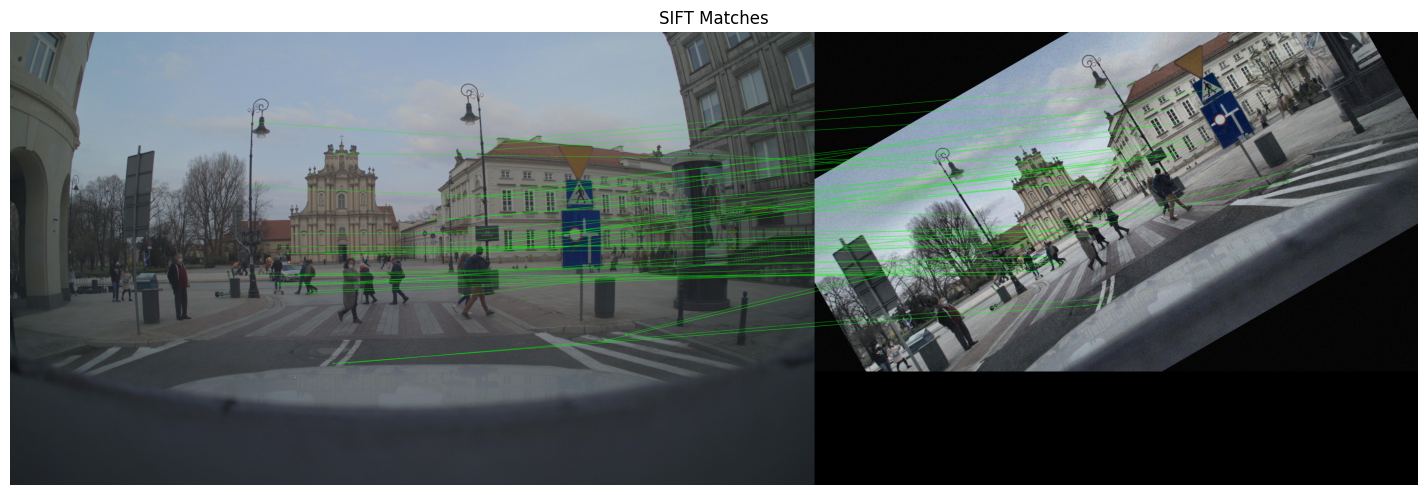
\includegraphics[width=0.6\textwidth]{images/matching_sift_complex.png}
    \caption{Visualización de matches entre imagen original y transformada compleja con SIFT.}
    \label{fig:matches_complex}
\end{figure}

\subsection{Matching con imagenes de referencia}

A partir de los resultados anteriores, hemos desarrollado una clase \texttt{SignMatcher}
que nos permite realizar el matching de señales de tráfico de referencia 
con imágenes de prueba. Esta clase permite cargar un conjunto de imágenes
de referencia, extraer sus descriptores locales y realizar el matching
con imágenes de prueba, devolviendo las localizaciones de las señales detectadas.

Respecto a la extracción de descriptores, hemos optado por utilizar SIFT, ya que
ha demostrado ser el método más estable de los 3 probados. Aun así, si se desease
un procesamiento en tiempo real, ORB sería la única opción viable.

Para los métodos de matching, se tienen disponibles dos opciones: matching
utilizando fuerza bruta. Es el método más exhaustivo y preciso, pero también
el más lento. El otro método disponible es FLANN (Fast Library for Approximate Nearest Neighbors),
que utiliza estructuras de datos avanzadas para acelerar el proceso de búsqueda
de vecinos más cercanos. FLANN es generalmente más rápido que la fuerza bruta,
aunque para descriptores de tan poco tamaño como los que manejamos, la diferencia
no es tan apreciable, por lo que hemos optado por utilizar fuerza bruta para
obtener la máxima precisión posible.

Para generalizar el matching a señales de distintos tamaños y posiciones en la imagen,
hemos importado imágenes de señales genéricas para utilizarlas como referencias.
La figura \ref{fig:sign_references} muestra las utilizadas.
\begin{figure}
    \centering
    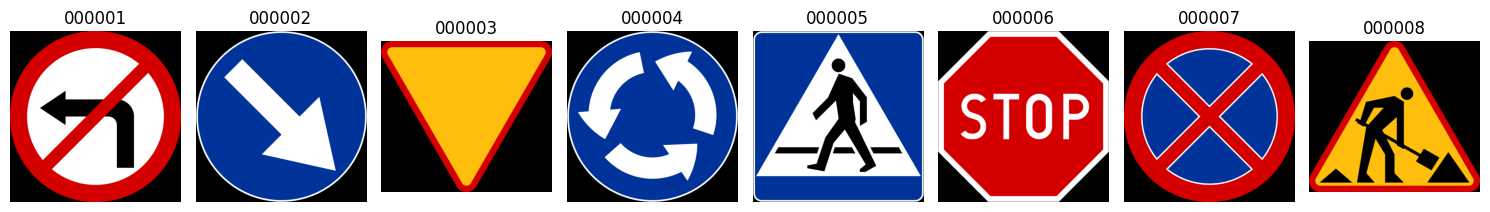
\includegraphics[width=0.6\textwidth]{images/sign_references.png}
    \caption{Imágenes de referencia utilizadas para el matching de señales.}
    \label{fig:sign_references}
\end{figure}

Inicialmente, los resutados son muy malos, ya que se está intentando
matchear toda la imagen de prueba con las imágenes de referencia, lo que
hace el resultado no tenga sentido. La imagen \ref{fig:bad_matching} muestra
un ejemplo de este mal resultado.

\begin{figure}
    \centering
    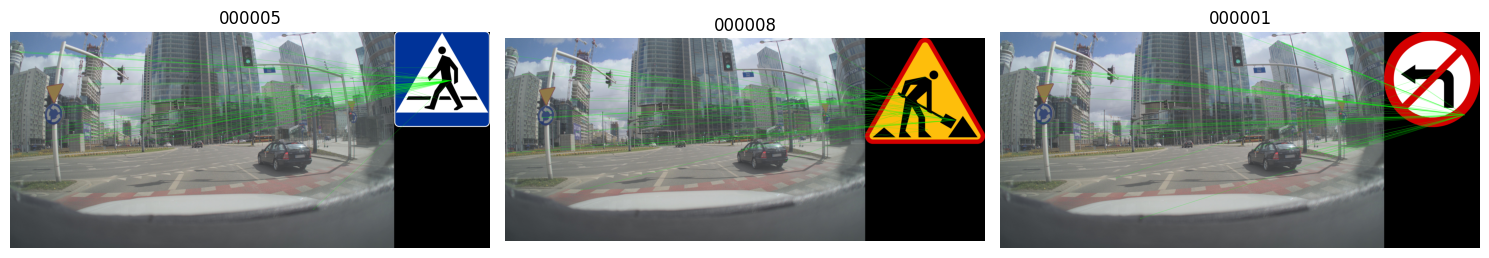
\includegraphics[width=0.6\textwidth]{images/bad_matching.png}
    \caption{Mal resultado de matching.}
    \label{fig:bad_matching}
\end{figure}

Es necesario aplicar RANSAC para hacer una estimación robusta de las
homografías a partir de los descriptores matcheados. Así se filtran
los matches incorrectos y se obtiene, teoricamente, una localización 
precisa de las señales. Véase en la figura \ref{fig:good_matching} un ejemplo
de un resultado de calidad mixta al aplicar RANSAC. La señal de paso de 
peatones es localizada correctamente, pero tenemos un 
falso positivo muy grande con la señal de stop.

\begin{figure}
    \centering
    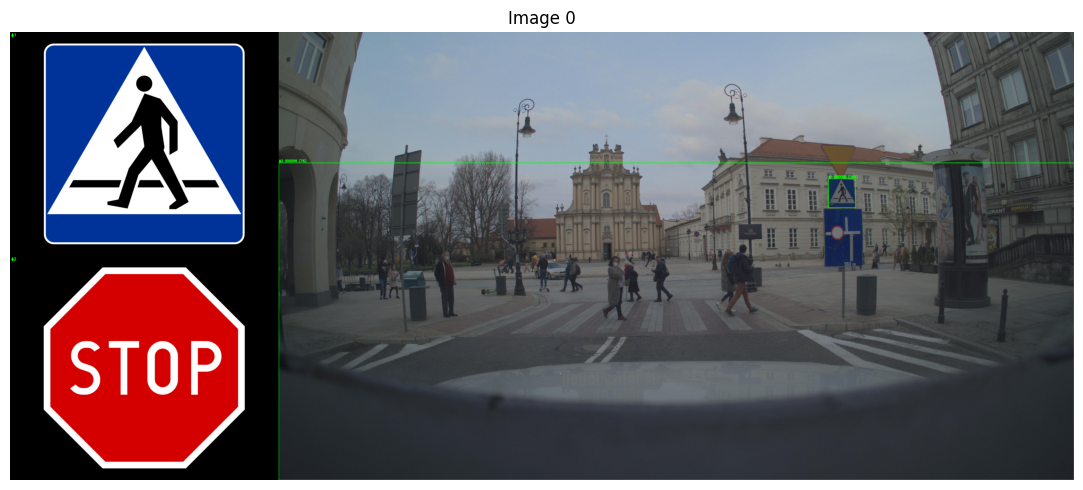
\includegraphics[width=0.6\textwidth]{images/good_matching.png}
    \caption{Resultado de matching con RANSAC.}
    \label{fig:good_matching}
\end{figure}

En el resto de imágenes con las que se ha probado, tambien ocurren resultados
parecidos o peores. Casi nunca logramos matchear ninguna señal correctamente,
y a menudo se producen falsos positivos muy grandes. Véase en las figuras \ref{fig:good_matching_2}
y \ref{fig:bad_matching_2} dos ejemplos adicionales de resultados obtenidos. En la primera
se identifica correctamente una señal, pero en la segunda no se identifica ninguna
señal correctamente.

\begin{figure}
    \centering
    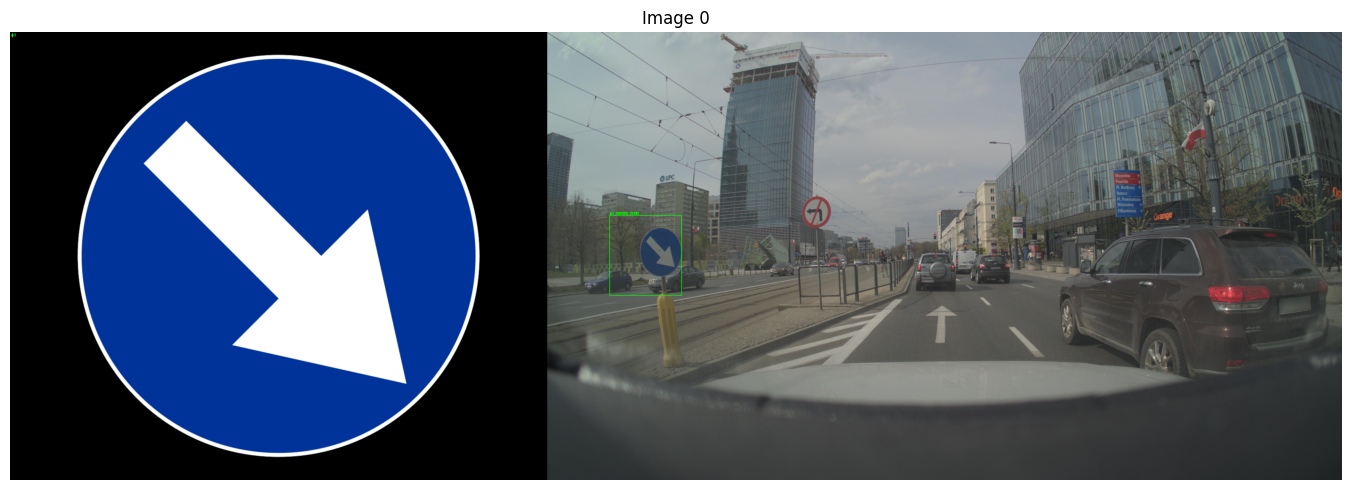
\includegraphics[width=0.6\textwidth]{images/good_matching2.png}
    \caption{Resultado de matching con RANSAC.}
    \label{fig:good_matching_2}
\end{figure}

\begin{figure}
    \centering
    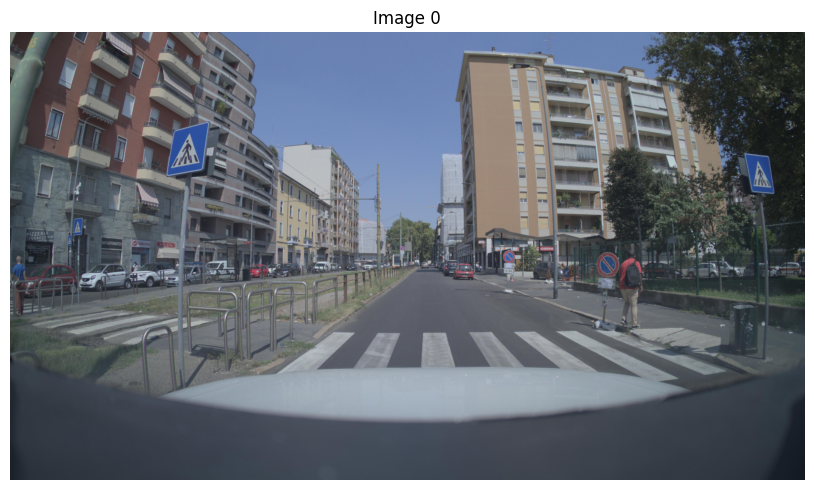
\includegraphics[width=0.6\textwidth]{images/bad_matching2.png}
    \caption{Resultado de matching con RANSAC.}
    \label{fig:bad_matching_2}
\end{figure}

Para intentar mejorar los resultados, vamos a intentar aplicar un preprocesamiento
de corrección de distorsión y de contraste dinámico. A partir del cual se ha visto como mejora un poco
los resultados en ciertas imágenes, véase como en la figura \ref{fig:preprocessed_matching}
se mejora la localización de la señal de paso de cebra, detectado además la de 
indicación de dirección obligatoria (aunque no muy bien posicionada). Aun así,
 muchísimas señales continuan sin ser detectadas, y los falsos positivos siguen siendo un problema. 

\begin{figure}
    \centering
    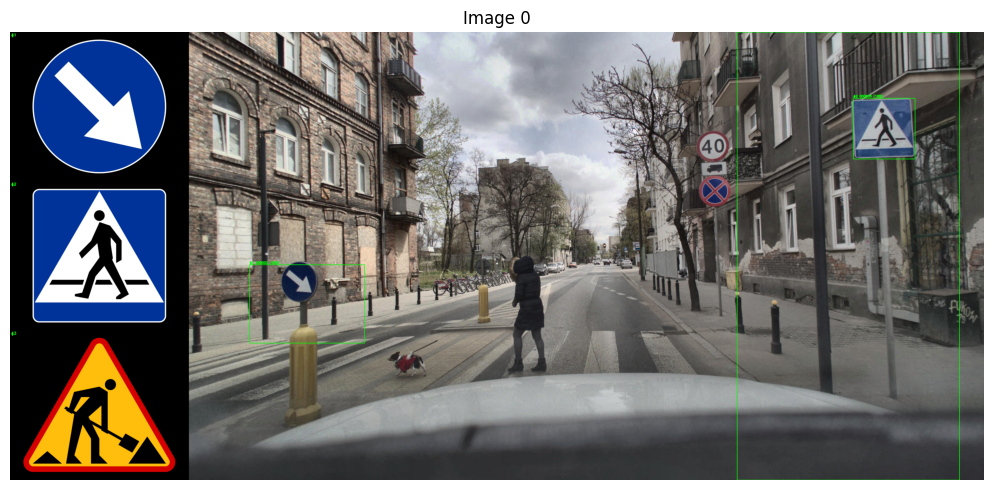
\includegraphics[width=0.6\textwidth]{images/contrast_good_match.png}
    \caption{Resultado de matching con RANSAC tras preprocesamiento.}
    \label{fig:preprocessed_matching}
\end{figure}

Como apunte adicional, para comprobar la correctitud de nuestra implementación,
hemos ejecutado el mismo proceso de matching usando como imágenes de prueba
las zonas recortadas de las señales del dataset, de esta forma se puede comprobar
si el método es capaz de matchear correctamente las señales recortadas a su imagen
de origen. En la figura \ref{fig:cropped_matching} se muestra un ejemplo de este experimento.

\begin{figure}
    \centering
    \begin{subfigure}[b]{0.45\textwidth}
        \centering
        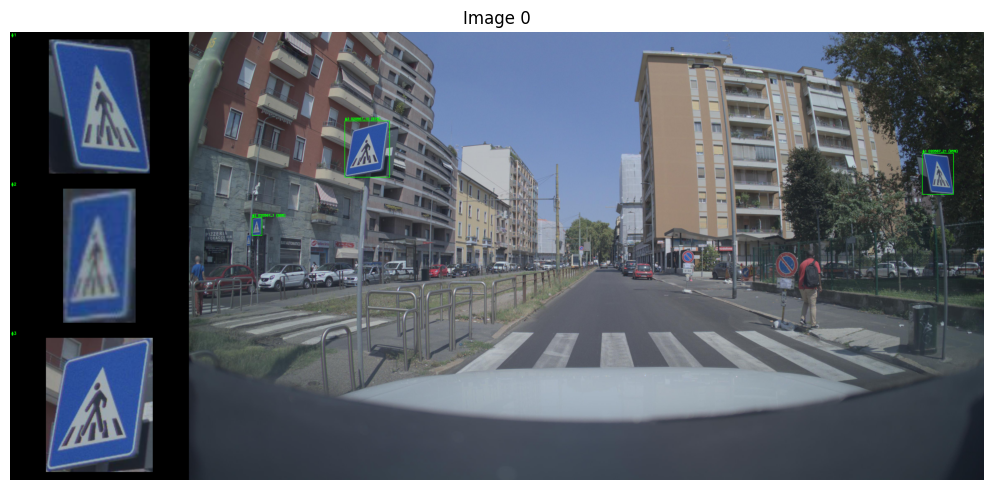
\includegraphics[width=\textwidth]{images/matches_cebras.png}
        \caption{Imagen recortada de señal.}
    \end{subfigure}
    \hfill
    \begin{subfigure}[b]{0.45\textwidth}
        \centering
        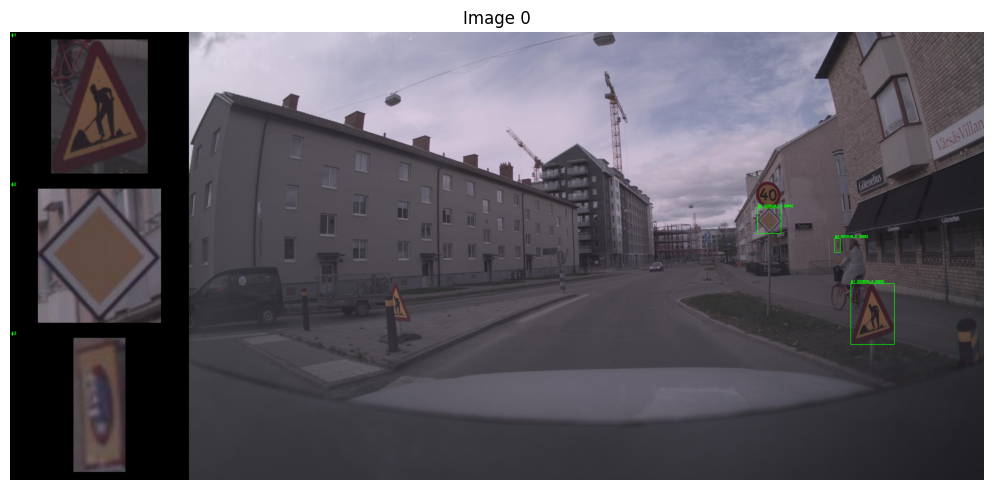
\includegraphics[width=\textwidth]{images/matches_obras.png}
        \caption{Resultado de matching con RANSAC.}
    \end{subfigure}
    \caption{Matching de imagen recortada de señal a su imagen de origen.}
    \label{fig:cropped_matching}
\end{figure}

Los descriptores locales (SIFT, AKAZE, ORB) con template matching, aunque efectivos para objetos 
texturados y transformaciones geométricas simples, presentan limitaciones significativas en la detección robusta de señales de tráfico en 
condiciones reales. El problema fundamental radica en que las señales reales sufren variaciones extremas de 
iluminación, desgaste, oclusiones parciales, reflejos y perspectivas diversas, mientras que las imágenes de referencia son
renders sintéticos o fotografías en condiciones controladas. Además, las señales de tráfico son objetos pequeños en escenas grandes con texturas 
limitadas (colores planos, bordes simples), generando pocos keypoints para matching robusto. El preprocesamiento puede intentar mitigar estas diferencias, 
pero no puede resolver el gap entre templates sintéticos y señales reales bajo condiciones adversas.

\subsection{Clasificador HOG para detección de señales}

\textit{Items de evaluación: \underline{\textbf{BT3kp}}.}

Ante las limitaciones observadas del template matching con descriptores locales, 
hemos implementado un clasificador basado en Histogramas de Gradientes Orientados (HOG)
combinado con una Máquina de Vectores de Soporte (SVM) lineal. Este enfoque creemos que es particularmente 
adecuado para la detección de objetos con formas estructuradas como las señales de tráfico.

El clasificador funciona mediante ventana deslizante: se recorre la imagen a múltiples 
escalas extrayendo parches de tamaño fijo (64$\times$64 píxeles), se calcula el descriptor HOG 
de cada parche, y se clasifica como señal o no-señal mediante el SVM entrenado.

\subsubsection{Algoritmo HOG implementado}

Hemos desarrollado una implementación propia del algoritmo HOG desde cero, siguiendo 
los pasos clásicos descritos por Dalal y Triggs\cite{dalal2005}:

\begin{enumerate}
    \item \textbf{Cálculo de gradientes}: Se aplican filtros Sobel con kernel de tamaño 1 
    para obtener las derivadas en X e Y de la imagen en escala de grises. A partir de 
    estos gradientes se calculan la magnitud y orientación de cada píxel:
    \begin{align}
        G_x &= \frac{\partial I}{\partial x}, \quad G_y = \frac{\partial I}{\partial y} \\
        m &= \sqrt{G_x^2 + G_y^2} \\
        \theta &= \arctan\left(\frac{G_y}{G_x}\right) \mod 180º
    \end{align}
    
    \item \textbf{Histogramas por celda}: La imagen se divide en celdas de 8$\times$8 píxeles. 
    Para cada celda se construye un histograma de 9 bins (orientaciones de 0° a 180°) 
    ponderado por la magnitud de los gradientes. Se utiliza interpolación bilineal 
    entre bins adyacentes para mayor robustez.
    
    \item \textbf{Normalización por bloques}: Se agrupan las celdas en bloques de 2$\times$2 
    y se concatenan sus histogramas. Cada bloque se normaliza usando L2-Hys: 
    primero normalización L2, luego recorte de valores a 0.2, y finalmente 
    re-normalización L2.
    
    \item \textbf{Vector de características}: Los bloques normalizados se concatenan 
    para formar el descriptor final. Para parches de 64$\times$64 píxeles con los parámetros 
    por defecto (9 orientaciones, celdas 8$\times$8, bloques 2$\times$2), esto resulta en un vector 
    de 1764 dimensiones.
\end{enumerate}

El entrenamiento del clasificador sigue el siguiente proceso:
\begin{itemize}
    \item \textbf{División de datos}: El conjunto de imágenes se divide en 80\% entrenamiento 
    y 20\% test de forma aleatoria pero reproducible (semilla fija).
    
    \item \textbf{Extracción de parches}: Para cada imagen de entrenamiento se extraen 
    parches positivos (de las ROIs anotadas) y negativos (regiones aleatorias sin 
    intersección con señales). Los ROIs grandes se particionan en sub-parches con 
    50\% de solapamiento.
    
    \item \textbf{Balanceo}: Se ajusta automáticamente el número de negativos para 
    mantener un ratio equilibrado con los positivos.
    
    \item \textbf{Clasificación}: Se entrena un SVM lineal sobre los descriptores HOG 
    normalizados (StandardScaler).
\end{itemize}

\subsubsection{Resultados con implementación skimage}

Presentamos primero los resultados utilizando la implementación de HOG de la 
librería scikit-image como referencia de rendimiento. La tabla \ref{tab:hog_skimage_patch}
muestra los resultados de clasificación a nivel de parches individuales etiquetados.

Para mantener la reproducibilidad, se ha fijado la misma semilla aleatoria en todas las ejecuciones
de todas las versiones evaluadas.

\paragraph{Métricas de clasificación a nivel de parche:}
\begin{table}[H]
    \centering
    \caption{Métricas de clasificación (parches)}
    \label{tab:hog_skimage_patch}
    \begin{tabular}{lcc}
        \toprule
        \textbf{Métrica} & \textbf{Train} & \textbf{Test} \\
        \midrule
        Accuracy & 0.722 & 0.755 \\
        Precision &  0.645 & 0.837\\
        Recall & 0.795 & 0.796\\
        F1-Score & 0.712 & 0.816 \\
        Muestras & 1600 & 401 \\
        \bottomrule
    \end{tabular}
\end{table}

Para un mejor análisis, se ha obtenido métricas de detección a nivel de imagen.
Para ello, seleccionando 25 imágenes aleatoriamente del conjunto de test, se ha aplicado
el clasificador en modo ventana deslizante, y se han comparado las detecciones
obtenidas con las anotaciones de señales reales. Los resultados se muestran en la tabla
\ref{tab:hog_skimage_detection}.

Tengase en cuenta que las clasificaciones no son resultados binarios,
sino que se obtiene una puntuación de confianza para cada ventana.
Se ha seleccionado un umbral de 0.5 para considerar una ventana como detección positiva.

\paragraph{Métricas de detección (ventana deslizante):}
\begin{table}[H]
    \centering
    \caption{Métricas de detección}
    \label{tab:hog_skimage_detection}
    \begin{tabular}{lc}
        \toprule
        \textbf{Métrica} & \textbf{Valor} \\
        \midrule
        True Positives & 1023 \\
        False Positives & 58095 \\
        True Negatives & 716573 \\
        False Negatives & 4409 \\
        Accuracy & 0.9201 \\
        Precision & 0.0173 \\
        Recall & 0.1883\\
        F1-Score & 0.0317\\
        Hit Rate & 0.9201\\
        GT Coverage & 0.1090\\
        \bottomrule
    \end{tabular}
\end{table}

Las métricas más significativas son el \textit{Hit Rate o accuracy} (porcentaje de clasificaciones
correctas sobre todas las ventanas clasificadas tanto positivas como negativas) y el \textit{GT Coverage}
(porcentaje de ventanas positivas correctamente detectadas sobre el total de señales reales).

\subsubsection{Resultados con implementación custom}

A continuación se presentan los resultados obtenidos con nuestra implementación 
propia del algoritmo HOG.

\paragraph{Métricas de clasificación a nivel de parche:}
\begin{table}[H]
    \centering
    \caption{Métricas de clasificación (parches).}
    \label{tab:hog_custom_patch}
    \begin{tabular}{lcc}
        \toprule
        \textbf{Métrica} & \textbf{Train} & \textbf{Test} \\
        \midrule
        Accuracy & 0.837 & 0.814\\
        Precision & 0.853 & 0.946\\
        Recall & 0.752 & 0.771\\
        F1-Score & 0.799 & 0.85\\
        Muestras & 1600 & 401 \\
        \bottomrule
    \end{tabular}
\end{table}

\paragraph{Métricas de detección (ventana deslizante):}
\begin{table}[H]
    \centering
    \caption{Métricas de detección}
    \label{tab:hog_custom_detection}
    \begin{tabular}{lc}
        \toprule
        \textbf{Métrica} & \textbf{Valor} \\
        \midrule
        True Positives & 640\\
        False Positives & 17873\\
        True Negatives & 758795\\
        False Negatives & 4792\\
        Accuracy & 0.971\\
        Precision & 0.035\\
        Recall & 0.118\\
        F1-Score & 0.054\\
        Hit Rate & 0.971\\
        GT Coverage & 0.071\\
        \bottomrule
    \end{tabular}
\end{table}

\paragraph{Comparación con skimage:}
\begin{table}[H]
    \centering
    \caption{Comparación de rendimiento skimage vs custom}
    \label{tab:hog_comparison}
    \begin{tabular}{lccc}
        \toprule
        \textbf{Métrica} & \textbf{skimage} & \textbf{custom} & \textbf{Diferencia} \\
        \midrule
        F1-Score (parches) & 0.816 & 0.85 & 0.034 \\
        F1-Score (detección) & 0.031 & 0.054 & 0.023 \\
        \bottomrule
    \end{tabular}
\end{table}

Se puede observar como nuestra implementación custom mejora ligeramente
los resultados obtenidos con la implementación de skimage, tanto a nivel
de parches como a nivel de detección en ventana deslizante. El lado negativo es que
en tiempo de cómputo nuestra implementación es considerablemente más lenta,
debido a que no hemos optimizado el código tanto como en la librería skimage.

\subsubsection{Resultados con preprocesado de imagen}

Finalmente, evaluamos el impacto de aplicar técnicas de preprocesado antes de 
la extracción de características HOG. Por simplicidad, se ha aplicado únicamente
el segmentado por color en espacio HSV expuesto en bloques anteriores.

\paragraph{Métricas de clasificación a nivel de parche:}
\begin{table}[H]
    \centering
    \caption{Métricas de clasificación (parches)}
    \label{tab:hog_preprocess_patch}
    \begin{tabular}{lcc}
        \toprule
        \textbf{Métrica} & \textbf{Train} & \textbf{Test} \\
        \midrule
        Accuracy & 0.803 & 0.772 \\
        Precision & 0.793 & 0.9131 \\
        Recall & 0.737 & 0.737 \\
        F1-Score & 0.764 & 0.816\\
        Muestras & 1600 & 401 \\
        \bottomrule
    \end{tabular}
\end{table}

\paragraph{Métricas de detección (ventana deslizante):}
\begin{table}[H]
    \centering
    \caption{Métricas de detección}
    \label{tab:hog_preprocess_detection}
    \begin{tabular}{lc}
        \toprule
        \textbf{Métrica} & \textbf{Valor} \\
        \midrule
        True Positives & 3527 \\
        False Positives & 215295 \\
        True Negatives & 561373 \\
        False Negatives & 1905 \\
        Accuracy & 0.722 \\
        Precision & 0.0161 \\
        Recall & 0.649\\
        F1-Score & 0.032 \\
        Hit Rate & 0.722 \\
        GT Coverage & 0.124 \\
        \bottomrule
    \end{tabular}
\end{table}

En esta versión con preprocesado, hemos intentado maximizar GT Coverage,
ya que queremos asegurarnos de detectar el mayor número posible de señales reales,
aunque a costa de aumentar los falsos positivos. Para ello se ha relajad el umbral
de detección a -0.3 (en lugar de 0.5 original). Aun así, el GT Coverage
mejora sólo un 2\% sobre el total respecto a la versión sin preprocesado.

\subsubsection{Imágenes de comparación}

A continuación se muestran algunas imágenes de ejemplo con los resultados
obtenidos con el clasificador HOG+SVM en modo ventana deslizante para las 
distintas versiones implementadas.

\begin{figure}
    \centering
    \begin{subfigure}[b]{0.45\textwidth}
        \centering
        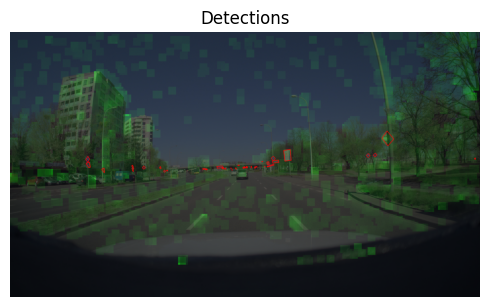
\includegraphics[width=\textwidth]{images/hog/skimage_1.png}
        \caption{HOG skimage}
    \end{subfigure}
    \hfill
    \begin{subfigure}[b]{0.45\textwidth}
        \centering
        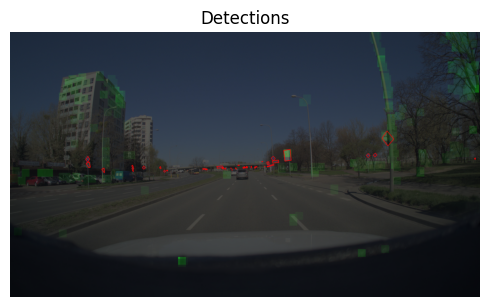
\includegraphics[width=\textwidth]{images/hog/custom_1.png}
        \caption{HOG custom}
    \end{subfigure}
    \hfill
    \begin{subfigure}[b]{0.45\textwidth}
        \centering
        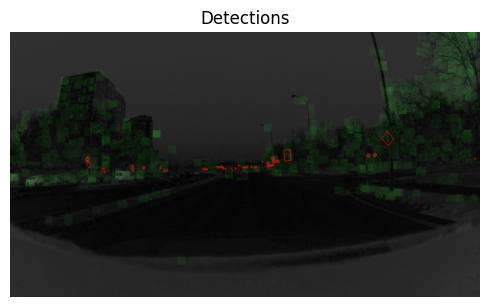
\includegraphics[width=\textwidth]{images/hog/pre_1.png}
        \caption{HOG con preprocesado}
    \end{subfigure}
    \caption{Comparación de resultados de detección con distintas versiones del clasificador HOG+SVM.}
    \label{fig:hog_comparison}
\end{figure}


\begin{figure}
    \centering
    \begin{subfigure}[b]{0.45\textwidth}
        \centering
        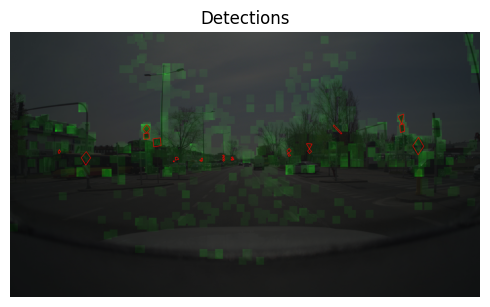
\includegraphics[width=\textwidth]{images/hog/skimage_2.png}
        \caption{HOG skimage}
    \end{subfigure}
    \hfill
    \begin{subfigure}[b]{0.45\textwidth}
        \centering
        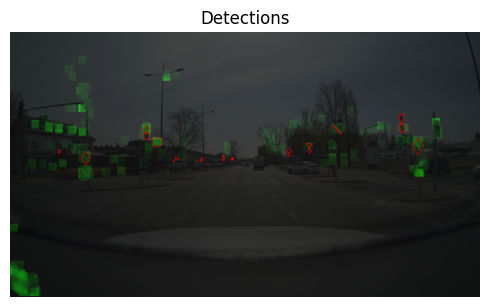
\includegraphics[width=\textwidth]{images/hog/custom_2.png}
        \caption{HOG custom}
    \end{subfigure}
    \hfill
    \begin{subfigure}[b]{0.45\textwidth}
        \centering
        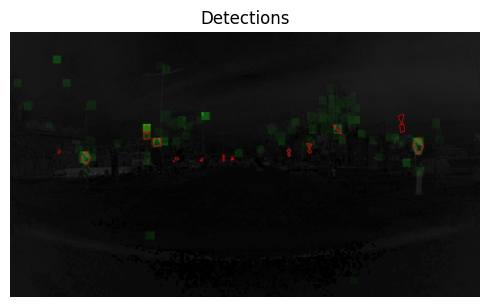
\includegraphics[width=\textwidth]{images/hog/pre_2.png}
        \caption{HOG con preprocesado}
    \end{subfigure}
    \caption{Comparación de resultados de detección con distintas versiones del clasificador HOG+SVM.}
    \label{fig:hog_comparison_2}
\end{figure}


\begin{figure}
    \centering
    \begin{subfigure}[b]{0.45\textwidth}
        \centering
        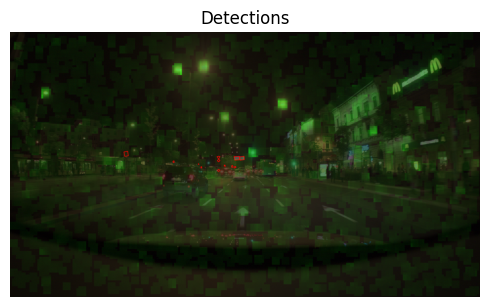
\includegraphics[width=\textwidth]{images/hog/skimage_3.png}
        \caption{HOG skimage}
    \end{subfigure}
    \hfill
    \begin{subfigure}[b]{0.45\textwidth}
        \centering
        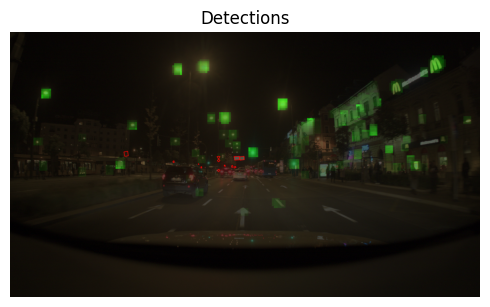
\includegraphics[width=\textwidth]{images/hog/custom_3.png}
        \caption{HOG custom}
    \end{subfigure}
    \hfill
    \begin{subfigure}[b]{0.45\textwidth}
        \centering
        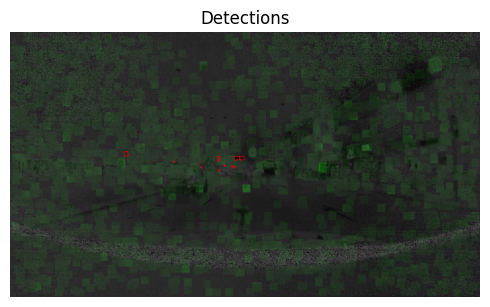
\includegraphics[width=\textwidth]{images/hog/pre_3.png}
        \caption{HOG con preprocesado}
    \end{subfigure}
    \caption{Comparación de resultados de detección con distintas versiones del clasificador HOG+SVM.}
    \label{fig:hog_comparison_3}
\end{figure}


\begin{figure}
    \centering
    \begin{subfigure}[b]{0.45\textwidth}
        \centering
        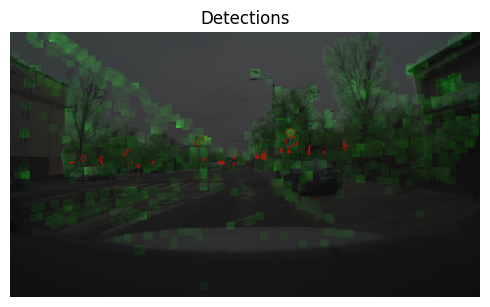
\includegraphics[width=\textwidth]{images/hog/skimage_4.png}
        \caption{HOG skimage}
    \end{subfigure}
    \hfill
    \begin{subfigure}[b]{0.45\textwidth}
        \centering
        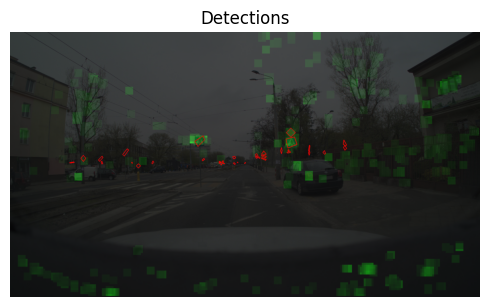
\includegraphics[width=\textwidth]{images/hog/custom_4.png}
        \caption{HOG custom}
    \end{subfigure}
    \hfill
    \begin{subfigure}[b]{0.45\textwidth}
        \centering
        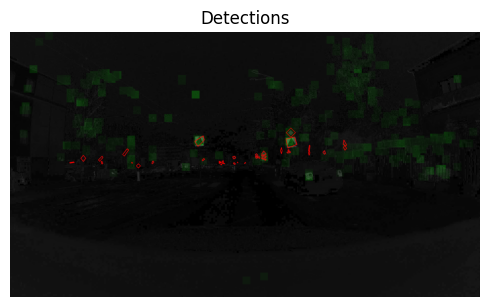
\includegraphics[width=\textwidth]{images/hog/pre_4.png}
        \caption{HOG con preprocesado}
    \end{subfigure}
    \caption{Comparación de resultados de detección con distintas versiones del clasificador HOG+SVM.}
    \label{fig:hog_comparison_4}
\end{figure}


\begin{figure}
    \centering
    \begin{subfigure}[b]{0.45\textwidth}
        \centering
        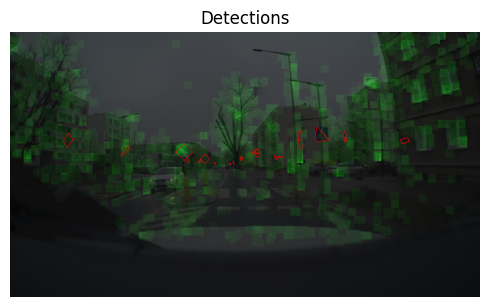
\includegraphics[width=\textwidth]{images/hog/skimage_5.png}
        \caption{HOG skimage}
    \end{subfigure}
    \hfill
    \begin{subfigure}[b]{0.45\textwidth}
        \centering
        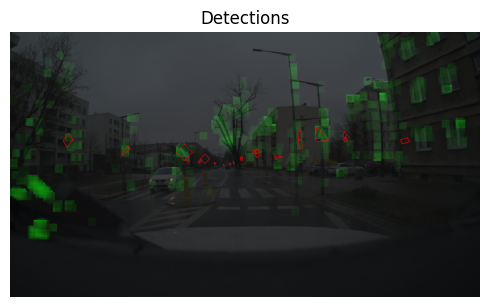
\includegraphics[width=\textwidth]{images/hog/custom_5.png}
        \caption{HOG custom}
    \end{subfigure}
    \hfill
    \begin{subfigure}[b]{0.45\textwidth}
        \centering
        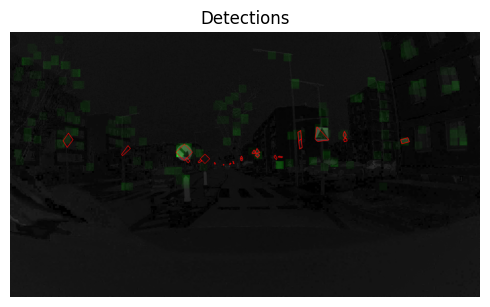
\includegraphics[width=\textwidth]{images/hog/pre_5.png}
        \caption{HOG con preprocesado}
    \end{subfigure}
    \caption{Comparación de resultados de detección con distintas versiones del clasificador HOG+SVM.}
    \label{fig:hog_comparison_5}
\end{figure}

\subsubsection{Conclusiones HOG}

Los resultados obtenidos tienen sentido dentro de las limitaciones del enfoque HOG+SVM
y atendiendo al dataset elegido. En las imágenes de muestra, se observa como podemos llegar a lograr
que se clasifique correctamente señales en primer plano y bien destadas. Sin embargo, el etiquetado
del que disponemos es quizas demasiado exhaustivo, incluyendo señales muy pequeñas, parcialmente ocluidas,
en condiciones adversas e incluso las de dirección contraria en las que sólo se ve el reverso.

Todo esto, en especial las limitaciones de tamaño y vista de reverso, puede provocar que el clasificador
confunda zonas de fondo de la imagen con señales reales, generando muchos falsos positivos.
Además, las señales pequeñas y ocluidas son difíciles de detectar incluso para un humano,
por lo que el clasificador no puede aprender a detectarlas correctamente.

A estas alturas, un enfoque basado en Deep Learning con una red neuronal convolucional
sería probablemente más adecuado para este problema, que se verá en el siguiente bloque de trabajo.

\section*{Uso de IA}

Se ha utilizado IA conversacional para asistencia en la elaboración de código y en la comprensión de los algoritmos. Todo el contenido generado fue revisado y adaptado por los autores.

\bibliographystyle{ieeetr}
\bibliography{references}

\end{document}